%!TEX root = ../report.tex
\documentclass[../report.tex]{subfiles}
\begin{document}
    \chapter{Conclusions}
	The previous chapter presented results of the conducted experiments and related analyses. This chapter concludes this thesis by listing its contributions, giving answers to the formulated research questions and providing directions to continue this research work in future.
	\section{Revisiting Research Questions}
	This section revisits the research questions formulated in Chapter \ref{ch_intro} and explains how they are answered in this research work.\\
	
	
	\textbf{RQ1.} What are the XAI methods to determine important regions in an input image for a CNN based classifier model to make its predictions?
	
	\textbf{A1:} The attribution class of methods is used to highlight regions in an input image, which are crucial for a CNN classifier model to make its predictions. Chapter \ref{ch_sota} presented a literature review of various attribution methods by categorizing them into three types: input, layer and neuronal. Three SOTA layer attribution methods (GradCAM, HiResCAM and FullGrad) were considered for conducting experiments related to this research work.\\
	
	\textbf{RQ2.} What are the key regions in frontal facial images fed to CNN models trained for the task of classifying rare genetic disorders?
	
	\textbf{A2:} Features in the nose region are predominantly considered by GestaltMatcher, a SOTA genetic syndrome classification model to recognize CDLS, WBS and HPMRS conditions. Layer-wise activation visualization (refer Section \ref{sec_layer_wise}) revealed that the model focuses on the lip region to recognize WBS. Results of the syndrome-wise attribution map experiment (refer Section \ref{sec_expc}) showed that down-slanting palpebral fissures feature is used to recognize instances of CSS. \\
	
	
	\textbf{RQ3.} How do the regions obtained from findings of RQ2 compare with the knowledge known to the medical community on facial phenotypes of the corresponding rare genetic syndromes?

	\textbf{A3:} Artifacts of experiments A, B and C belonging to three syndrome categories (CDLS, WBS and HPMRS) were evaluated by an experienced clinical geneticist. Regions considered important by GestaltMatcher to recognize CDLS and HPMRS matched with those of the clinician. In particular, both considered eyebrow and nasal regions to recognize the syndromes. On the other hand, there was a mismatch observed in the regions considered to identify WBS. Looking into OMIM, a knowledge base on rare-genetic syndromes and their associated features, enabled us to identify the nasal region to contain discriminative features for recognizing rare genetic conditions (refer Section \ref{sec_inf}).
	
    \section{Contributions}
	Following is the list of important contributions made by this work:
	\begin{itemize}
	\item Literature review and identification of SOTA XAI methods suitable to explain predictions of the GestaltMatcher model.
	\item Integration of the shortlisted methods with GestaltMatcher and related fine-tuning.
	\item Generation of patient-wise and syndrome-wise attribution maps, and composite faces for all 139 frequent classes in the GMDB dataset.
	\item Formulation of an evaluation procedure for the generated artifacts.
	\item Realization of the evaluation procedure in the form of a questionnaire (available on Google forms\footnote[1]{Questionnaire - \url{https://forms.gle/aRru9aeCyZaqpURP9}}).
	\item Analysis of results obtained from an experienced clinician's evaluation of experimental artifacts, representing three classes (CDLS, WBS and HPMRS) in GMDB dataset.
	\item Identification of the nose region as a discriminative feature to recognize rare genetic conditions.
	\item Experimentation to analyze the effects of dataset imbalance on the quality of attribution maps.
	\item Contribution to a publication\footnote[2]{F. Brand, A. Vijayananth, T.-C. Hsieh, A. Schmidt, S. Peters, E. Mangold, K. Cremer, T. Bender,
		S. Sivalingam, H. Hundertmark et al., “Next-generation phenotyping contributing to the identification
		of a 4.7 kb deletion in kansl1 causing koolen-de vries syndrome,” Human Mutation, vol. 43, no. 11,
		pp. 1659–1665, 2022.} in \textit{Human Mutation }journal, based on the findings of this research work (refer Appendix \ref{ch_contributions}).
	\item Presentation of a research poster in the annual meeting of AGDev\footnote[3]{https://www.agdev.de/tagung2022.html}(refer Appendix \ref{ch_contributions}).
	\end{itemize}
	\section{Lessons learned}
	The following insights were gained during the course of this research work:
	\begin{itemize}
	\item Whenever possible, it is a better choice to use an inherently interpretable machine learning model over black boxes like neural networks, for high stake applications.
	\item Each attribution method aims to explain a particular aspect of a neural network prediction. GradCAM, for example, approaches attribution as \enquote{weakly supervised localization}, while perturbation methods represent the magnitude of change in the classifier score, when an input image is manipulated. Therefore, it is prudent to choose XAI method based on the task at hand over other reasons.
	\item Attribution methods need to be used in conjunction with other classes of XAI methods to explain predictions of models. 
	\item Even experienced clincians find diagnosis of rare genetic syndromes to be a challenging task.
	
	\item There is a definite need to develop a common framework for the scientific community to evaluate XAI methods on aspects like meaningfulness and usability.
	
	\item XAI methods have the potential to yield novel insights about the data and model with which they are used.
	\end{itemize}
    \section{Future work}
    \begin{figure}[H]
    	\centering     
    	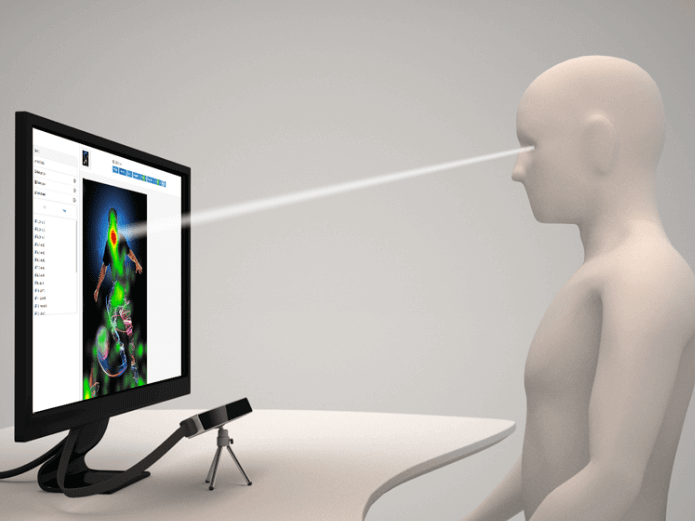
\includegraphics[scale=0.4]{eye_tracking.png}
    	\caption{A typical eye tracking setup. Image source: uxbooth\protect\footnotemark}
    	\label{fig_eye_track}
    \end{figure}
	\footnotetext[1]{uxbooth - https://www.uxbooth.com/articles/a-look-into-predictive-eye-tracking-tools/}
    This section provides future directions of research related to this work:
    \begin{itemize}
    	\item  During the course of this research work, we realized the need to associate regions highlighted in attribution maps with those considered important by the clinician evaluating them, in a quantitative way. An eye tracking setup such as the one shown in Figure \ref{fig_eye_track}, could be used to track the evaluator's eye movements, determine his/her regions of attention on the displayed patient's facial image. Gaze maps obtained from eye-tracking, could be compared with attribution maps by computing the overlap between their highlighted regions, interms of metrics like intersection over union (IOU) \footnote[2]{IOU}. The comparison is valid under the assumption that duration of the evaluator's gaze on a particular region is directly proportional to its importance for syndrome recognition. 
    	\item The GestaltMatcher framework proposes the use of cosine similarity metric to quantitatively compare images of patients from same or different syndromes in the clinical face phenotype space (CFPS). However, cosine similarity such measured, is a scalar value which does not reveal any information about the regions of similarity or differences between a given pair of facial images. Applying attribution methods such as GradCAM, on a siamese network \cite{taigman2014deepface} model trained on pairs of images along with their cosine similarity scores  in CFPS, might reveal the regions of similarity between an inputted pair of images. If successful, such an XAI would aid the scientific community to accelerate its research on rare genetic syndromes and their associated phenotypes.
    	\item  One of the important findings of this research work is the importance of the nasal region in the recognition of rare genetic conditions. This could be used as an empirical evidence by the research community to search for novel gene-phenotype associations.
    
    \end{itemize}
\end{document}
